% =========================================================
% CONFIGURACION DEL DOCUMENTO
% =========================================================
\providecommand{\main}{..}
\documentclass[../main.tex]{subfiles}

% =========================================================
% CONTENIDO
% =========================================================
\begin{document}

\chapter{Componentes del Sistema}\label{Componentes del Sistema}

En el presente capítulo se presentan los componentes que constituyen el quadrotor y su sistema de control e instrumentación, como así también los soportes para realizar las pruebas experimentales de estabilización por eje.


\section{Componentes para la implementación del controlador}

Para implementar la estrategia de control desarrollada en los capítulos
anteriores, se comienza por describir el hardware y los soportes utilizados
para realizar los pruebas preliminares de control sobre subsistemas
y posteriormente, de acuerdo con el desempeño logrado, asegurar la
estabilidad de la planta completa.


\subsection{Controlador }

Ni myRIO-1900 es un dispositivo portable y reconfigurable diseñado
especialmente para proyectos con fines académicos de control, robótica
y mecatrónica. Este dispositivo cuenta con varios tipos de entrada
y salida análogas, digitales y audio, comunicación inalámbrica, procesador
en tiempo real y FPGA programable. 

\begin{figure}[H]
\noindent \begin{centering}
\includegraphics[scale=0.7]{\string"NI myRIO Hardware Diagram\string".jpg}
\par\end{centering}
\caption{Diagrama de Hardware NI myRIO 1900.}
\end{figure}

\textcompwordmark{}

En la siguiente tabla se resumen las características de consumo del
controlador myRIO 1900.

\begin{table}[H]
\noindent \begin{centering}
\begin{tabular}{|c|c|}
\hline 
Modelo & myRIO 1900\tabularnewline
\hline 
\hline 
Voltaje Funcionamiento & 6-16 {[}VDC{]}\tabularnewline
\hline 
Consumo Máximo & 14 {[}W{]}\tabularnewline
\hline 
Consumo Típico & 2.6 {[}W{]}\tabularnewline
\hline 
Procesador & Xilinx Z-7010\tabularnewline
\hline 
Velocidad del Procesador & 667 {[}MHz{]}\tabularnewline
\hline 
Memoria No Volatil & 256 {[}Mb{]}\tabularnewline
\hline 
Memoria DDR3 & 512{[}Mb{]}, 533{[}MHz{]}, 16 bits.\tabularnewline
\hline 
Wireless & IEEE 802.11, ISM 2.4 {[}GHz{]}, AnchoBanda 20 {[}MHz{]}\tabularnewline
\hline 
USB Ports & USB 2.0 Hi-Speed\tabularnewline
\hline 
Pines Entradas Análogas  & 8 de 0-5{[}V{]}, 2 de $\pm$10{[}V{]}\tabularnewline
\hline 
Pines Salidas Analógicas  & 4 de 0-5{[}V{]}, 4 de $\pm$10{[}V{]}\tabularnewline
\hline 
Pines de E/S Digitales & 30 de 0-5{[}V{]} (6 PWM, 4 ENC, 2 UART, 2 I2C, 2 SPI)\tabularnewline
 & 7 de $\pm$10{[}V{]} (2 PWM, 4 ENC)\tabularnewline
\hline 
Entradas Audio & 2 de $\pm$2.5{[}V{]}\tabularnewline
\hline 
Acelerómetro & 3 ejes, $\pm$8 {[}g{]}, 12 bits, 800 {[}S/s{]}, 3.9 mg rms 25 [$\degree$C]\tabularnewline
\hline 
\end{tabular}
\par\end{centering}
\caption{Especificaciones NI myRIO 1900.}
\end{table}

\textcompwordmark{}

\begin{figure}[H]
\noindent \begin{centering}
\subfloat[{E/S digitales y análogas 0-5 {[}V{]}.}]{\noindent \begin{centering}
\includegraphics[scale=0.48]{\string"pines 0-5 volts\string".jpg}
\par\end{centering}
}\subfloat[{E/S digitales y análogas $\pm$10 {[}V{]}.}]{\noindent \begin{centering}
\includegraphics[scale=0.52]{\string"pines 10 volts\string".jpg}
\par\end{centering}}
\par\end{centering}
\caption{E/S NI myRIO 1900.}
\end{figure}


\subsection{Marco del Vehículo}

Para el desarrollo experimental existen varios tipos de marcos para
el armado de un quadcopter, diferentes tamaños y materiales. Para
éste proyecto se utiliza el marco $Turnigy\ Talon\ V2\ Quadcopter$,
el cual está hecho de fibra de carbono, ofreciendo a la vez resistencia,
peso ligero y buen aspecto estético. Las placas de montaje de los
motores permiten montarlos en dos posiciones y permiten tamaños diferentes.
El sistema de sujeción del recuadro central cuenta con el tamaño apropiado
para asegurar una buena fijación de los brazos. Resultado de las pruebas
de estrés del diseño hechas por el fabricante, es que el marco puede soportar hasta 5{[}kg{]}
de carga en el centro con mínima deformación en cada brazo. 

\begin{figure}[H]
\noindent \begin{centering}
\includegraphics[scale=0.6]{\string"Estructura\string".pdf}
\par\end{centering}
\caption{Recuadro central y posición de motores en estructura Turnigy Talon
V2.}
\end{figure}

Las principales ventajas del marco son su forma y rigidez, dado que
uno de los supuestos para el control es la simetría y rigidez del
marco. Cabe destacar también la durabilidad de la estructura, las
placas compatibles con motores de diferente tamaño, la carga máxima
que soporta, lo que otorga bastante holgura para la implementación.
Las principales desventajas son el tamaño del recuadro central, dado
que el controlador a utilizar excede en tamaño a dicho recuadro, dificultando
la fijación al vehículo.

\subsection{Motores, Controladores de Velocidad y Hélices.}

Los motores a utilizar son motores brushless sensorless, que como
su nombre lo dice, no cuentan con escobillas. En este tipo de motor
la parte móvil es donde se encuentran los imanes permanentes, y en
la parte fija o estator, se encuentran los bobinados conductores.
Para el funcionamiento de éste tipo de motores se necesita de un controlador
electrónico (ESC) que envíe pulsos alternados al circuito trifásico
a partir de una señal PWM en su entrada. 

\textcompwordmark{}

\begin{table}[H]
\noindent \begin{centering}
\begin{tabular}{|c|c|}
\hline 
\multicolumn{1}{|c}{Modelo } & NTM Prop Drive Series 30-35A\tabularnewline
\hline 
\hline 
Kv & 1100{[}rpm/v{]}\tabularnewline
\hline 
Corriente Máxima & 32{[}A{]}\tabularnewline
\hline 
Voltaje Máximo & 16.8{[}V{]}\tabularnewline
\hline 
Potencia Máxima & 380{[}W{]}@15{[}V{]} (4S)\tabularnewline
\hline 
ESC (Controlador) & 40\tabularnewline
\hline 
Peso & 88{[}g{]}\tabularnewline
\hline 
Diametro & 35{[}mm{]}\tabularnewline
\hline 
Altura Total & 32{[}mm{]}\tabularnewline
\hline 
Batería & Lithium Polymer Battery 3s\textasciitilde{}4s\tabularnewline
\hline 
\end{tabular}
\par\end{centering}
\caption{Especificaciones Motores Brushless NTM Prop Drive Series 35-30A.}
\end{table}

\begin{figure}[H]
\noindent \begin{centering}
\subfloat[{Motor Brushless NTM Propdrive 35-30 1100 {[}kv{]}}]{\noindent \begin{centering}
\includegraphics[scale=0.27]{\string"NTM3530\string".jpg}
\par\end{centering}
}\subfloat[{Programmable Brushless ESC Hobbyking 30 {[}A{]}. }]{\noindent \begin{centering}
\includegraphics[scale=0.3]{\string"ESC\string".jpg}
\par\end{centering}}
\par\end{centering}
\caption{Actuadores.}
\end{figure}


Por sus siglas en inglés ESC (Electric Speed Controler), es un dispositivo
que se encarga de controlar la velocidad de los motores eléctricos brushless. Ésto lo realiza por medio de una señal electrica PWM de
50{[}Hz{]} enviada desde el controlador myRIO-1900, la cual dependiendo
de su ciclo de trabajo regula los pulsos enviados hacia el motor trifásico
para aumentar o reducir la velocidad angular de éstos. En el Anexo D
se incluye la configuración de estos dispositivos, la cual incluye
características programables como el tipo de aceleración, la forma
de frenado de los motores, la frecuencia de los pulsos, etc.

\begin{table}[H]
\noindent \begin{centering}
\begin{tabular}{|c|c|}
\hline 
\multicolumn{1}{|c}{Modelo } & HobbyKing Programmable ESC HK3A\tabularnewline
\hline 
\hline 
Corriente Máxima & 40{[}A{]}\tabularnewline
\hline 
Voltaje Máximo & 16.8{[}V{]}\tabularnewline
\hline 
Peso & 32{[}g{]}\tabularnewline
\hline 
Dimensiones & 54/26/11{[}mm{]}\tabularnewline
\hline 
Batería & Lithium Polymer Battery 3s\textasciitilde{}4s\tabularnewline
\hline 
\end{tabular}
\par\end{centering}
\caption{Especificaciones del controlador de velocidad.}
\end{table}

\textcompwordmark{}

Las hélices se pueden caracterizar por medio de dos parámetros: el
paso y el diámetro. El primero determina cuanto avanzaría la hélice
al girar si estuviera en un medio que no deslizara, similar al movimiento
de un tornillo o tuerca, mientras que el diámetro es el tamaño de
la hélice de un extremo a otro. 

\begin{figure}[H]
\noindent \begin{centering}
\includegraphics[scale=0.5]{\string"helice diametro y paso diagrama\string".jpg}
\par\end{centering}
\caption{Paso y Diámetro de Hélices.}
\end{figure}

Cabe mencionar que existen casos donde se opta por utilizar hélices
de paso variable, como así también hélices de más de
dos aspas [16], pero como el vuelo acrobático y maniobras
complejas no son parte de los objetivos de éste trabajo, se opta por
escoger hélices de paso fijo. Su dimensión es 10'' de diámetro y 4.5'' de paso. 
El empuje y torque producido por el conjunto motor-hélice se describe en el Capítulo de Modelado de la Planta y se caracteriza en el Capítulo de Simulación.


\subsection{Sensores}

Para la implementación del sistema se deben medir los ángulos $ \phi, \theta, \psi $ de inclinación
y orientación del vehículo. Para ésto se combinan las mediciones de
un acelerómetro y gyróscopo utilizando un filtro complementario. Los
sensores que se utilizan en la implementación son el acelerómetro
incorporado en el controlador myRIO-1900 y el gyróscopo ITG3200 incluido
en la unidad de medición inercial 9dof Sensor Stick de Sparkfun. Las
características principales de ambos sensores se describen en las
siguientes tablas.

\begin{table}[H]
\noindent \begin{centering}
\subfloat[Gyroscopo ITG-3200]{\noindent \begin{centering}
\begin{tabular}{|c|c|}
\hline 
Gyróscopo & ITG3200\tabularnewline
\hline 
\hline 
Voltaje de Entrada & 2-3.6 {[}V{]} DC\tabularnewline
\hline 
Ejes  & 3\tabularnewline
\hline 
Comunicación & I2C\tabularnewline
\hline 
Rango máximo & $\pm$2000 {[}$\degree$ /s{]}\tabularnewline
\hline 
Resolución & 16 bits\tabularnewline
\hline 
Frecuencia de Muestreo & 3.9 - 8000 {[}Hz{]}\tabularnewline
\hline 
Ruido  & 0.38 {[}$\degree$ /s rms{]}\tabularnewline
\hline 
\end{tabular}
\par\end{centering}}
\par\end{centering}
\noindent \begin{centering}
\subfloat[Acelerómetro integrado en controlador myRIO-1900]{\noindent \begin{centering}
\begin{tabular}{|c|c|}
\hline 
Acelerómetro & myRIO-1900 Accel\tabularnewline
\hline 
\hline 
Voltaje de Entrada & Integrado en myRIO-1900\tabularnewline
\hline 
Ejes & 3\tabularnewline
\hline 
Comunicación & Integrado en myRIO-1900\tabularnewline
\hline 
Rango máximo & $\pm$8 {[}g{]}\tabularnewline
\hline 
Resolución & 12 bits \tabularnewline
\hline 
Frecuencia de Muestreo & 800 {[}Hz{]}\tabularnewline
\hline 
Ruido & 3.9 {[}mg rms{]} at 25 {[}$\degree$ C{]}\tabularnewline
\hline 
\end{tabular}
\par\end{centering}}
\par\end{centering}
\caption{Características de sensores para la implementación.}
\begin{comment}
Preguntar al Profesor Fernando que más puede ser relevante en la descripción
de las características.
\end{comment}
\end{table}

Para verificar el correcto funcionamiento de la adquisición de datos y estimación del ángulo de inclinación y orientación del vehículo, se utiliza un programa de pruebas con visualización en 3D que es descrito en el Capítulo de Instrumentación y Control.


\begin{figure}[H]
\noindent \begin{centering}
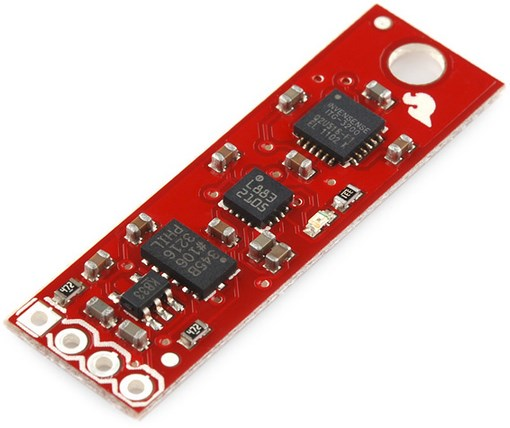
\includegraphics[scale=0.27]{IMU}
\par\end{centering}
\caption{Sparkfun 9dof IMU, gyróscopo ITG-3200.}
\end{figure}

\textcompwordmark{}

\subsection{Batería}

Existen varios tipos de baterías que se utilizan en los vehículos
aéreos no tripulados de vuelo interior. En primer lugar se tienen
las baterías de niquel cadmio $Ni-Cd$, este tipo de baterías cuentan
con efecto memoria, el cual se produce cuando se recarga la batería
sin haberla descargado por completo con anterioridad, impidiendo su
recarga a máxima capacidad. Luego dada la toxixidad del cadmio, se
comenzaron a utilizar baterías de níquel metal hidruro $Ni-Mh$, las
que no poseen efecto memoria, contienen menos contaminantes y poseen
una mayor capacidad, pero menor número de recargas. También se cuenta
con baterias de iones de litio $Li-ion$, las que duplican la capacidad
de las baterías de niquel cadmio, no poseen efecto memoria, pero necesitan
un limitador del voltaje máximo de cada celda. Por último se tienen
las baterías de polímeros de litio $Li-Po$, las cuales poseen mas
de 5 veces la capacidad de las baterías de $Ni-Mh$, son ligeras,
no poseen restricciones en su forma, no poseen efecto memoria y son
ideales para alimentar motores. La desventaja que poseen, es el tiempo
de recarga respecto a los otros tipos mencionados debido a su mayor
capacidad. A pesar de esta desventaja, se selecciona éste tipo de
baterías, puesto que la capacidad y peso son de mayor importancia
que el tiempo de recarga.

En la siguiente tabla se describen las principales características
de la batería seleccionada para la alimentación de los motores.

\begin{table}[H]
\noindent \begin{centering}
\begin{tabular}{|c|c|}
\hline 
\multicolumn{1}{|c}{Modelo:} & Turnigy 5000mAh 4S 30C Lipo\tabularnewline
\hline 
\hline 
Capacidad  & 5000{[}mAh{]}\tabularnewline
\hline 
Configuración & 4S1P / 14.8{[}v{]} / 4Cell\tabularnewline
\hline 
Constante de Descarga & 30C\tabularnewline
\hline 
Peso & 556{[}g{]}\tabularnewline
\hline 
Ancho & 36{[}mm{]}\tabularnewline
\hline 
Largo & 144{[}mm{]}\tabularnewline
\hline 
Alto & 49{[}mm{]}\tabularnewline
\hline 
\end{tabular}
\par\end{centering}
\caption{Especificaciones bateria Turnigy 3000mAh 3S 30C Lipo.}
\end{table}

\begin{figure}[H]
\noindent \begin{centering}
\includegraphics[scale=1.4]{\string"battery lipo 5000mah\string".jpg}
\par\end{centering}
\caption{Batería LiPo Turnigy 5000{[}mah{]} 30C.}
\end{figure}

\textcompwordmark{}

\subsection{Soportes}

Para poder realizar las pruebas experimentales de la estabilización
de los ejes del quadcopter uno a la vez, se diseñan dos soportes.
Uno con el fin de realizar las pruebas de estabilización de forma
más cercana a como se comportaría el vehículo en vuelo hovering, mientras
que el otro es un soporte diseñado para que rote sobre los tres ejes
simultaneamente sujetando el vehículo en todo momento. El primero
es construido por el estudiante y el material escogido es madera,
mientras que el otro se manda a diseñar bajo el concepto del funcionamiento
de una junta cardánica. En las siguientes imágenes se pueden apreciar
ambos soportes y más adelante se describen el tipo de pruebas realizadas
sobre cada uno. 

\begin{figure}[H]
\noindent \begin{centering}
\subfloat[{Soporte de Metal 3DOF.}]{\noindent \begin{centering}
\includegraphics[scale=0.1]{\string"sopF\string".jpg}
\par\end{centering}
}\subfloat[{Soporte de Madera 1DOF}]{\noindent \begin{centering}
\includegraphics[scale=0.1]{\string"sopM\string".jpg}
\par\end{centering}}
\par\end{centering}
\caption{Soportes para pruebas de estabilización.}\label{Soporte de Maderita}\noindent
\end{figure}


\end{document}